\documentclass[12pt]{notes}

% Command for Questions
%\question{}

% Command for Notes
% \note{}

% Code to create a minipage where you can type in class notes. 
%%\begin{minipage}[l][2cm][c]{\textwidth}
\begin{comment}

\end{comment}
%%\end{minipage}


% Begin Document
%==============================================================================
\begin{document}
% Include the Title of the Handout
\ntitle{5.1: Logistic Regression}

% Include Numbered Sections
\section{Why Logistic Regression?}

Recall the linear regression model
$$Y = \beta_0 + \beta_1X_1 + \cdots + \beta_{p-1}X_{p-1} + \epsilon \qquad (\epsilon \sim N(0, \sigma^2)).$$

\question{(Individual) What are some properties of the variable $Y$ that are required for $\epsilon$ to be normally distributed.}

\begin{minipage}[l][3cm][c]{\textwidth}
\begin{comment}
\note{\bi
\item $Y$ must be linearly related to $X_1, \ldots X_{p-1}.$
\item $Y$ must be a \textbf{continuous, quantitative} variable
\ei}
\end{comment}
\end{minipage}

\subsection{Why not regression on categorical data?}
Consider fitting a regression model where we use age to try and predict whether or not a person has a disease (a 0-1 variable). 

\begin{figure}[H]
\centering
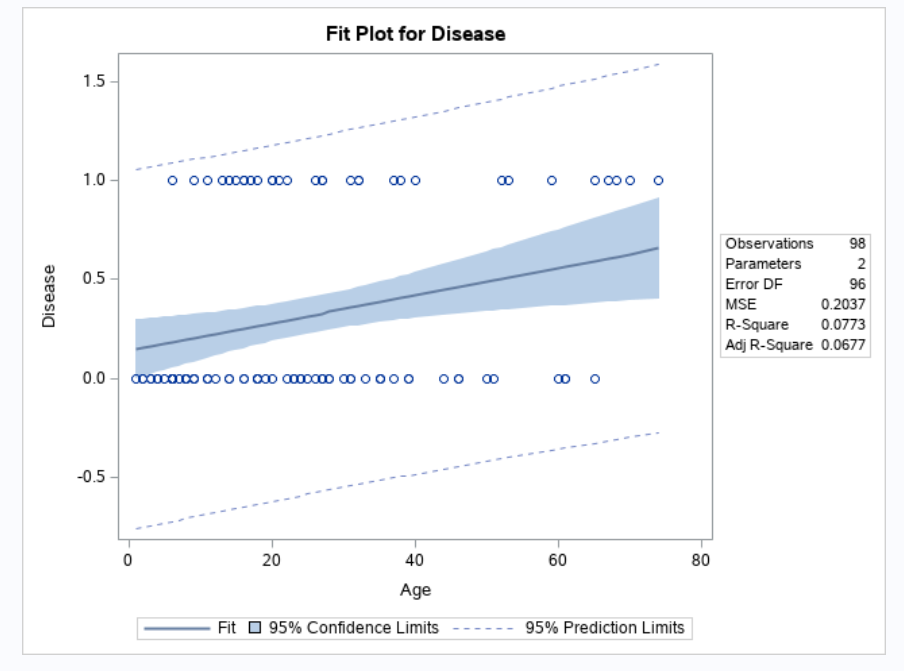
\includegraphics[width = 0.49\textwidth]{figures/module5/reg_resid.png}
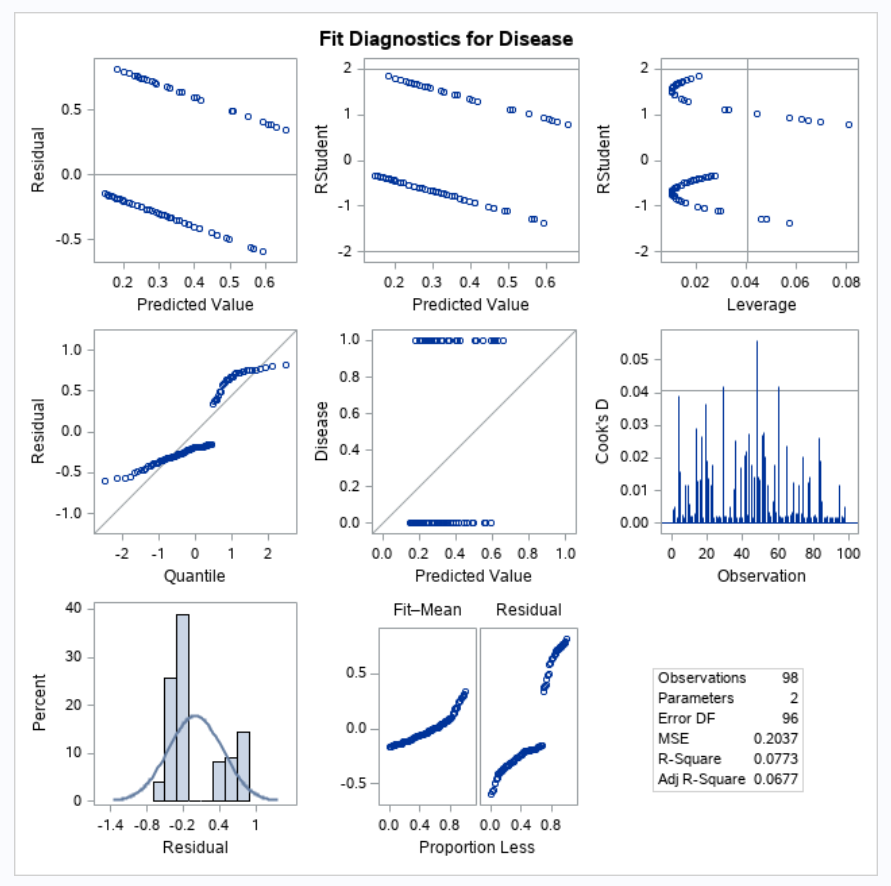
\includegraphics[width = 0.49\textwidth]{figures/module5/reg_resid2.png}
\caption{Fit plot and residual diagnostics for regression model that uses age to predict the presence/absence of a disease.}
\end{figure}

\nspace
It is for this reason that instead of trying to predict the \textbf{value} of a categorical predictor, we should rather try to predict the \textbf{probability} of occurrence $\pi_i$,
\begin{equation}
\pi_i = \beta_0 + \beta_1X_{i, 1} + \cdots + \beta_{p-1}X_{i, p-1} + \epsilon_i \qquad (\epsilon \sim N(0, \sigma^2)).
\label{eq:badreg}
\end{equation}

\nspace
\question{(Individual) However, based on the previous example, what are some of the issues with trying to predict the probability using (\ref{eq:badreg})?}

\begin{minipage}[l][3cm][c]{\textwidth}
\begin{comment}
\note{
\bi
\item We don't actually know $\pi_i$. 
\item Model can predict negative probabilities or probabilities above 1. 
\item Residual assumptions never satisfied (impossible for residuals to be normally distributed). 
\ei
}
\end{comment}
\end{minipage}

\section{Transforming Probabilities}
Because regression works best with \textbf{unconstrained} variables (i.e. variables that can theoretically take on any value). We need to find a transformation that maps $\pi \in [0, 1]$ to $f(\pi) \in (-\infty, \infty)$. 

\nspace
\textbf{Solution: log-odds ratio.}
\bi
\item $\pi \rightarrow [0,1]$
\item $\frac{\pi}{1-\pi} \rightarrow [0, \infty)$
\item $L = \log\left(\frac{\pi}{1-\pi}\right) \rightarrow (-\infty, \infty)$ 
\ei

\nspace
The \textbf{probit} function is another common transformation that achieves similar results. 
\bi
\item Probit: $Q_i = Z_{\pi_i} \rightarrow$ Z score (of a standard normal distribution) associated with the percentile $\pi_i$.  
\ei

\nspace
Other ``S'' shape curves exist, which tend to reach similar conclusions. 

\begin{figure}[H]
\centering
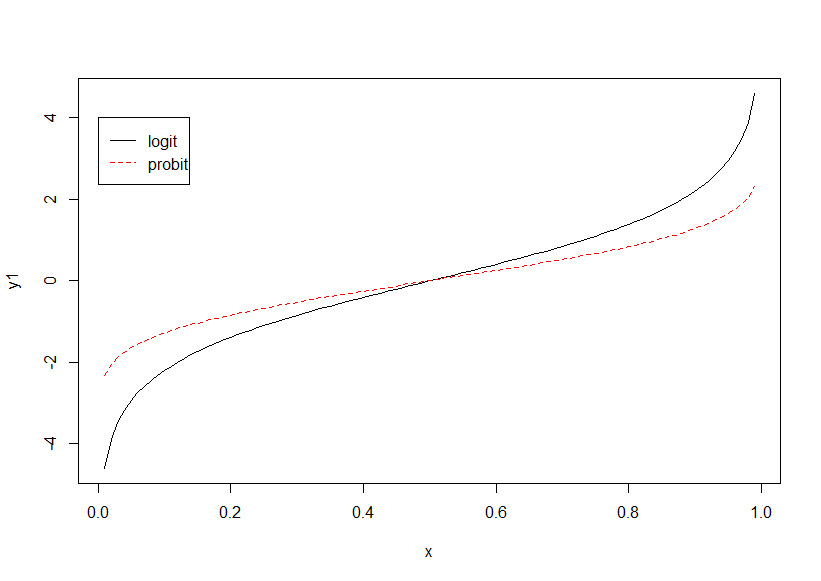
\includegraphics[width = 0.75\textwidth]{figures/module5/logit_probit.png}
\caption{Visualization of logit and probit function for various probabilities.}
\end{figure}

\section{Logistic Regression}

$$L_i = \beta_0 + \beta_1X_{i, 1} + \cdots + \beta_{p-1}X_{i, p-1} + \epsilon_i$$

\bi
\item $b_k$ estimates obtained from MLE-based iterative procedure (Newton-Raphson, Fisher)
\item Transform estimates $\hat{L}_i = b_0 + b_1X_{i, 1} + \cdots + b_{p-1}X_{i, p-1}$ back to probability scale. 
$$\hat{\pi}_i = \frac{1}{1+e^{-\hat{L}_i}} \qquad \qquad \hat{Odds}_i = e^{\hat{L_i}}$$
\ei

\subsection{Interpretation of Estimates}
\bi
\item $X_{i, 1} = \cdots = X_{i, p-1} = 0 \implies \hat{L}_i = b_0 \implies \hat{Odds}_i = e^{b_0}$
\item Hold $X_{i, 2} = \cdots = X_{i, p-1} = 0$, increase $X_{i, 1}$ from 0 to 1
$$\implies \hat{L}_i = b_0+b_1 \implies \hat{Odds}_i = e^{b_0 + b_1} = e^{b_0}e^{b_1}$$
\item Thus, an increase in one unit in $X_j$ \textit{multiplies the odds} (in favor of $Y=1$) by a factor of $e^{b_j}.$
\bi
\item Note that it is the \textit{odds} that are multiplied, \textbf{not} the probability. 
\ei
\item Alternative Interpretation: the odds of $Y=1$ change by $100(e^{b_j} - 1)\%$ per unit increase in $X_j$ while holding other predictors constant. 
\bi
\item Example (Handout 5.1.1): $b_j$ for sector is $1.57 \implies e^{1.57} = 4.83.$ 
\item ``Holding all other predictors constant, the odds of having disease are $100(4.83-1) = 383\%$ greater in Sector 2 than in Sector 1. 
\ei
\ei

\question{(Groups) How would you interpret the coefficient associated with Age in the Handout 5.1.1 logistic model?}

\begin{minipage}[l][2cm][c]{\textwidth}
\begin{comment}
\note{ ``Holding all other predictors constant, the odds of having disease are $100(e^{0.297} - 1) = 3.01\%$ greater for each year increase in age.''}
\end{comment}
\end{minipage}

\bi
\item The ``Odds Ratio'' for $X_j$ (odds of $Y=1$ when $X_j + 1$ vs odds of $Y=1$ when $X_j$)
$$\frac{e^{b_0 + b_1X_1 + \cdots + \mathbf{b_j(X_j + 1)} + \cdots + b_{p-1}X_{p-1}}}{e^{b_0 + b_1X_1 + \cdots + \mathbf{b_j(X_j)} + \cdots + b_{p-1}X_{p-1}}} = e^{b_j}$$
\ei

\subsection{Inference with Estimates}
\bi
\item Single Variable Test:
\bi
\item $H_0: \beta_j = 0$ ($X_j$ has no effect on $P(Y=1)$). 
\item Test statistic: $t = \frac{b_j}{SE\{b_j\}}$ (standard normal for ``large'' N). 
\item $\implies t^2 \sim \chi^2_1$ (obtain confidence intervals from here)
\bi
\item This approach is called the ``Wald Test''
\ei
\ei
\item Subset variables test:
\bi
\item $H_0: \beta_{p-H} = \cdots = \beta_{p-1} = 0$
\bi
\item reorder the X variables so that the subset we are checking for comes last
\ei
\item Let $L_{full}$ be the likelihood associated with the full model
\item Test statistics: $\chi^2 = -2\log\frac{L_{red}}{L_{full}}$
\item Under $H_0: \chi^2 \sim \chi^2_H$
\ei
\item Overall model test:
$$\text{Model} \chi^2 = -2\log L_{intercept} + 2\log L_{int \& covariates}$$
\bi
\item Often called the \textbf{deviance}, $DEV$ or $DEV(X_0, X_1, X_{p-1})$
\ei
\item Conditional Effect plot: predicted $\hat{\pi}$ vs one predictor $X_j$
\bi
\item While holding all other predictors at some constant level. The default level in SAS is the mean (average) of each variable. 
\ei
\ei

\section{Goodness of Fit Measures:}
\bi
\item Pseudo R-square: $\frac{\chi^2}{\chi^2 +n}$ ($\chi^2$ from model test)
\item Hosmer-Lemeshow Goodness of Fit Test
\bi
\item $H_0:$ logistic regression response function is appropriate 
\item Based on sorted $\hat{\pi}$ values, group observations into 5-10 roughly equal sized groups. 
\item Within each group, look at the total observed numbers of $Y=1$ and $Y=0$
\item Based on the model fit, calculate the total \textit{expected} numbers of $Y=1$ and $Y=0$. 
\item Test statistic $\chi^2$ is sum (across groups) of $\frac{(observed - expected)^2}{expected}$
\ei
\item ``Concordance'' - look at all pairs of observations with different $Y$
\bi
\item Let $n_c$ be the \# of ``concordant'' pairs (observed $Y=1$ has larger $\hat{\pi}$)
\item Let $n_d$ be the \# of ``discordant'' pairs (observed $Y=1$ has smaller $\hat{\pi}$)
\item Let $n_t$ be the \# of ``tied'' paired (observed $Y=1$ and $Y=0$ have same $\hat{\pi}$ (likely due to identical X-profiles)
\item Define rank correlation indices (larger is better):
\begin{align*}
\text{Somers' }D &= \frac{n_c - n_d}{n_c+n_d+n_t} \\
\\
\gamma &= \frac{n_c-n_d}{n_c + n_d} \\
\\
\text{Tau-a} &= \frac{n_c - n_d}{0.5(n-1)n} \\
\\
\text{AUC} &=  \frac{n_c + 0.5n_t}{n_c+n_d+n_t} 
\end{align*}
\ei
\item ROC (Receiver Operating Characteristic) Curve
\bi
\item Sort all observations from the smallest to biggest $\hat{\pi}.$
\item At each position in the list:
\bi
\item Use $\hat{\pi}$ as threshold for $\hat{Y} = 1$, moving cutoff from the standard 0.5 threshold. 
\item Calculate sensitivity: (proportion $Y_i=1$ values with $\hat{Y}_i = 1$).
\item Calculate specificity: (proportion $Y = 0$ values with $\hat{Y} = 0$). 
\bi
\item Sensitivity and Specificity - think smoke alarms and pregnancy tests. 
\ei
\item False positive rate (prop $Y=0$ values with $\hat{Y} = 1$) = 1 - specificity
\item Plot false positives against true positive rates (sensitivity)
\item Calculate the area under the curve. 
\ei
\ei
\ei


\question{Given the three ROC curves in Figure \ref{fig:ROC}, which model has the best predictive power and why?}

\begin{figure}[H]
\centering
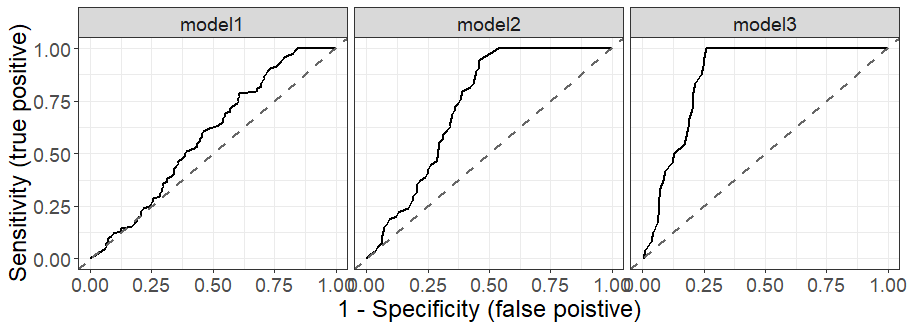
\includegraphics[width = \textwidth]{figures/module5/roc_curves.png}
\caption{Comparison of three ROC curves.}
\label{fig:ROC}
\end{figure}


\begin{minipage}[l][2cm][c]{\textwidth}
\begin{comment}
\note{Model 3 is the most accurate. The model sensitivity increases much faster than the false positive rate.}
\end{comment}
\end{minipage}

 
\section{Multicollinearity}
Recall that multicollinearity occurs when X variables are highly correlated with each other. It has \textbf{nothing} to do with the response variable $Y.$

\nspace
As in OLS, multicollinearity inflates the variance of the $b_k$ estimates, making them hard to interpret/test for significance.

\nspace
As in OLS, stepwise selection and all possible regression methods exist to ``score'' each combination of explanatory variables and select a best model. 



\section{Outliers in Logistic Regression}
\question{(Individual) If Y can only take on two values (0 or 1), how are outlier values possible?}

\begin{minipage}[l][2cm][c]{\textwidth}
\begin{comment}
\note{An outlier is a point for which the observation strongly disagrees with the predicted probability.}
\end{comment}
\end{minipage}

\bi
\item Define ``deviance residual'' as 
$$dev_i = \text{sign}(Y_i - \hat{\pi}_i)\sqrt{-2\left(Y_i\log\hat{\pi}_i + (1-Y_i)\log(1-\hat{\pi}_i)\right)}$$
\bi
\item The more certain we are (probability near 0 or 1), the more potential we have to be very wrong. 
\ei
\item $DEV(X_0, \cdots X_{p-1}) = \sum_i dev_i^2$
\item ``Outliers'' are values not well represented by the model
\item ``Half-normal probability plot - observed $|dev_i|$ vs expected value under normality
\bi
\item \textbf{However,} since the residuals are not normally distributed, we asses differences from our expectation using simulations based on $\hat{\pi}_i$. 
\bi
\item Create 19 simulations by generating a ``new'' response variable where the values of $Y_{new, i} \sim Bernoulli(\hat{\pi}_i)$
\ei
\item Simulated envelop (SEE 5.1.1 MACRO ON CANVAS) plots the minimum, maximum, and mean of the 19 simulations
\bi
\item Why 19 simulations? - Since our observed deviances represent the 20th observation, the probability that our deviances will fall outside the envelope is less than 5\% IF the fitted model is appropriate. 
\item Points falling outside in the envelop in the upper right corner of the plot are evidence of outliers/bad fits. 
\ei
\ei
\ei

\section{Influential Observations}
\nspace
Influential observations have the same effect on model coefficients as they did in OLS. 

\nspace
Diagnostics (similar to Leverage and DFBETAS):
\bi
\item $\Delta D_i: DEV - DEV_{(i)}$
\bi
\item Measures decrease in ``misfit'' when obs. $i$ is ignored. (essentially measures the ``poorness of fit for observation $i$). 
\item ``large'' $\Delta D_i \implies$ obs. $i$ overly influences model fit
\item SAS: DIFDEV - on step difference in deviance 
\ei
\item $\Delta B_i$
\bi
\item Similar to Cook's distance, measures influence of obs. $i$ on the estimates $b_j$
\item SAS: C - confidence interval displacement C
\ei
\item $\Delta \chi^2_i$
\bi
\item Similar to $\Delta D_i$: ``poorness of fit'' for obs $i$
\item SAS: DIFCHISQ - one step difference in Pearson $\chi^2$
\ei
\ei

\nspace 
Unlike in OLS, there is no consistent numerical rule of thumbs to determine thresholds for the $\Delta$ measures. 

\nspace
Instead, we will simply rely on graphical diagnostics. 
\bi
\item $\Delta D_i, \Delta B_i, \Delta X_i^2$ vs Observation Number - look for extreme values 
\item $\Delta D_i$ vs $\hat{\pi}_i$ (or $\Delta X_i^2$ vs $\hat{\pi}_i$)
\bi
\item Look for points with low $\hat{\pi}$ but $Y_i = 1$ (upper left corner) OR high $\hat{\pi}$ but $Y=0$ (upper right corner) which are much different than the overall pattern
\item (Optional) plot different size points where point size is determined by $\Delta B_i$
\ei
\ei

\section{Remedial Measures}
Similar to OLS:
\bi
\item Look for typos in the data
\item Consider transformations of the $X$ variables
\item Consider dropping problematic points (only if you have a good argument for removing them). 
\ei

\begin{comment}
\section{Origins of ``Logistic Regression}
\bi
\item If $T \sim Logistic(\mu, \beta)$, then the cumulative distribution function (CDF) of $T$ is $$F_T(t) = \frac{1}{1+e^{(-t+\mu)/\beta}}$$
\item CDF if called the ``logistic equation''
\bi
\item From the French ``equation logistique''
\item It is the solution to a particular differential equation related to population growth: $\frac{dP}{dt} = P(1-P), \, P(0) = 0.5$
\ei
\ei
\end{comment}


\section{Final Thought}
If you have a lot of explanatory variables, you should strongly consider classification trees and random forest for classification. 






















% End the Document
%==============================================================================
\end{document}